\documentclass{beamer}

\usepackage[frenchb]{babel}
\usepackage[T1]{fontenc}
\usepackage[utf8]{inputenc}

\definecolor{vertmoyen}{rgb}{0.25,0.45,0.10}


\usetheme{Berlin}

\setbeamercolor{structure}{fg=vertmoyen}
\setbeamertemplate{itemize item}[circle]

\setbeamertemplate{navigation symbols}{%
\hyperlink{sommaire}{\beamerreturnbutton{sommaire}}  
}

\title{
    Projet Système\\
    Compression Sans Perte
}
\author{Rémi GATTAZ - Julian HATTINGUAIS - Germain LECORPS - Reatha TITH}
\date{\today}

\begin{document}


\begin{frame}
\maketitle
\end{frame}

\begin{frame}
\tableofcontents
\end{frame}

\section{Cahier des Charges}

\begin{frame}
\begin{itemize}
\item Réversibilité
\item Marche pour tout fichier
\item Compresse selon les données du fichier
\item Prétraitement RLE
\item Possibilité de debug et traçage (trace très lourde pour les gros fichiers)
\item Temps de compression correct
\item Commandes faciles a utiliser
\end{itemize}
\end{frame}

\section{Organnisation}

\begin{frame}
\begin{itemize}
\item Première journée de conception (aucunes lignes de code)
\item Conception des différents modules (dico, binio, compression, décompression...)
\item Répartition du travail en binôme
\end{itemize}
\end{frame}


\section{LZW}

\subsection{Construction du dictionnaire}
\begin{frame}
 Besoins :
 \begin{enumerate}
  \item Compression : Arbre
  \item Décompression : Tableau
 \end{enumerate}
\end{frame}

\begin{frame}
 struct\_arbre $\{$ \newline
	char valeur; \newline
	Arbre* enfant; \newline
	Arbre* frere; \newline
	Arbre* parent; \newline
	Code code; \newline
$\};$
\end{frame}
\begin{frame}

struct\_dict $\{$ \newline
	int nbElements;	\newline	
	int tailleDico;	\newline	
	Arbre** ids;	\newline	
	Arbre* dico;	\newline	
$\};$

\end{frame}


\subsection{Binio}
\begin{frame}
 binio -> traitement des fichiers\newline
 \newline
 Utilisation d'un buffer :\newline
 \newline
 typedef struct s\_buffer $\{$ \newline
	char* content; \newline
	char* courant; \newline
	int significatif; \newline
	int longeur; \newline
$\}$ Buffer;
 
\end{frame}


\section{Prétraitement}

\subsection{Run Length Encoding}

\begin{frame}
Le codage se fait avec un automate à 2 états. On compare à chaque fois l'élément courant à l'élément précédent : si les deux sont égaux, on passe dans l'état 2 en incrémentant un compteur.
Le résultat du codage est de la forme suivante :\\
	$$abbbbcddddd -> 1a4b1c5d$$
Ainsi, pour un fichier où il y a peu de redondance, nous ajoutons un "1" devant chaque élément\\
Paquets max de 255
\end{frame}


\section{Commandes utiles}


\begin{frame}
- getopt\newline
- norme gnu\newline
Exemples :
    \begin{enumerate}
    \item ./LZW -c<file>
    \item ./LZW --compress=<file> -r
    \item ./LZW --rle -d<name>
    \item ./LZW --decompress=<file>
    \end{enumerate}
\end{frame}

\section{Tests}

\begin{frame}
    \begin{figure}[h]
    \centering
    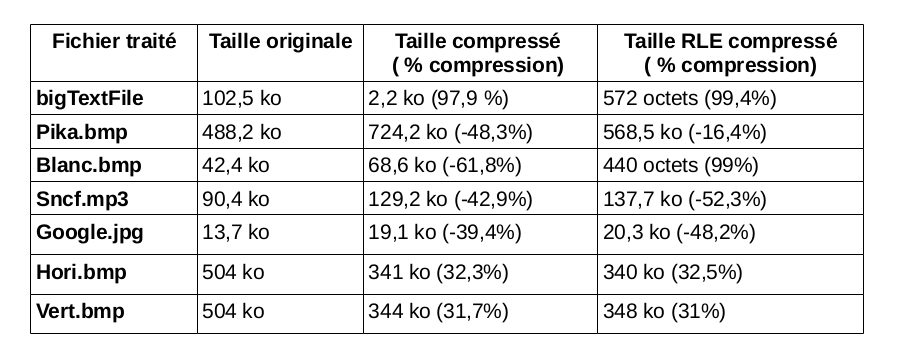
\includegraphics[scale=0.35]{tableau.png}
    \caption{Résultats pour différents fichiers et taux de compression}
    \label{resultats}
    \end{figure}
\end{frame}


\section{Problèmes rencontrés et évités}
\subsection{Difficultés}
\begin{frame}
 \begin{enumerate}
  \item Réinitialisation du dico
  \item Détection des erreurs de binio (test\_binio)
 \end{enumerate}
\end{frame}

\subsection{Facilités}
\begin{frame}
 \begin{enumerate}
  \item Répartition du travail (0 merge conflicts)
  \item Bonne conception
  \item Possiblité de changer de taille de dico très facilement
 \end{enumerate}
\end{frame}



\end{document}
